% Sean Anderson, 2012, sean@seananderson.ca
\documentclass[12pt]{article}
\usepackage{geometry}
\geometry{letterpaper}
\usepackage{graphicx}
\usepackage{grffile}
\usepackage{caption}

\renewcommand{\figurename}{Figure}

% A bit bigger than one inch margins:
\topmargin -1.43cm
\oddsidemargin 0.2cm
\evensidemargin 0.2cm
\textwidth 16.1cm
\textheight 22.75cm

\title{Lobster-temperature-predator figures}
\author{Sean Anderson}
%\date{}

%\setlength\parskip{0.1in}
%\setlength\parindent{0in}

%\thispagestyle{empty}
\pagenumbering{gobble}

\begin{document}
%\maketitle

\begin{figure}[htbp]
  \centering
    \includegraphics[height=3in]{map-colour.pdf}
  \caption{}
  \label{fig:lobmap.pdf}
\end{figure}

\begin{figure}[htbp]
  \centering
    \includegraphics[height=7in]{hom-time-series-effort.pdf}
  \caption{}
  \label{fig:home-ti}
\end{figure}

% \begin{figure}[htbp]
%   \centering
%     \includegraphics[height=4.5in]{rma_with_non_BLUPS.pdf}
%   \caption{Random effect meta-analysis without covariates. This will be redone
%   in base graphics to look better.}
%   \label{fig:rma_with_non_BLUPS.pdf}
% \end{figure}

%\begin{figure}[htbp]
%  \centering
%    \includegraphics[height=4in]{lme.ind.models.pred.nao.temp-withsgl.pdf}
%  \caption{From an old analysis, but here as a placeholder for how the previous
%  figure can look.}
%  \label{fig:lme.ind.models.pred.nao.temp-withsgl.pdffilename}
%\end{figure}
\begin{figure}[htbp]
  \centering
    \includegraphics[height=7in]{meta_analytic_curves.pdf}
    \caption{}
  \label{fig:meta_analytic_curves.pdf}
\end{figure}

\begin{figure}[htbp]
  \centering
    \includegraphics[height=6in]{meta_analytic_curves_effort.pdf}
  \caption{}
  \label{fig:ind.predators.corrs.pdf}
\end{figure}



\begin{figure}[htbp]
  \centering
    \includegraphics[height=4.0in]{ind.predators.corrs.pdf}
  \caption{}
  \label{fig:ind.predators.corrs.pdf}
\end{figure}

\clearpage

\begin{figure}[htbp]
  \centering
    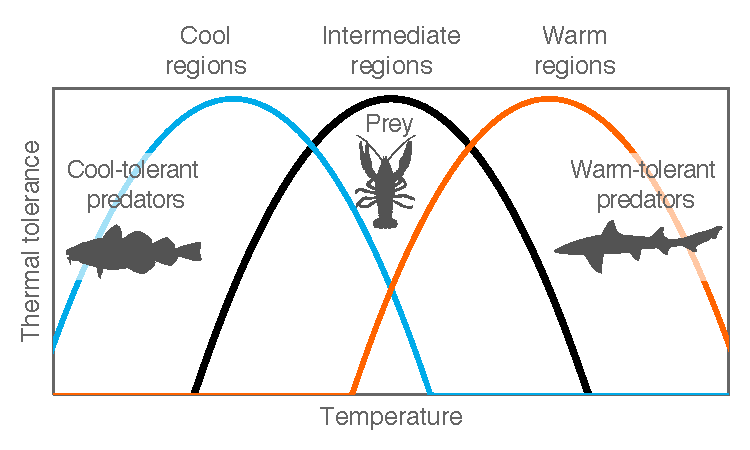
\includegraphics[height=2.5in]{optimal-curves-simple.pdf}
  \caption{}
  \label{fig:ind.predators.corrs.pdf}
\end{figure}


\renewcommand{\thefigure}{S\arabic{figure}}
\renewcommand{\figurename}{Figure}
\setcounter{figure}{0}  % reset counter

\begin{figure}[htbp]
  \centering
    \includegraphics[height=4.5in]{scaled_pred_abundance.pdf}
  \caption{REPLACE THIS WITH REAL FIG S1: landings abundance correlations}
  \label{fig:ind.predators.corrs.pdf}
\end{figure}

\begin{figure}[htbp]
  \centering
    \includegraphics[height=4.5in]{scaled_pred_abundance.pdf}
  \caption{}
  \label{fig:ind.predators.corrs.pdf}
\end{figure}

\begin{figure}[htbp]
  \centering
    \includegraphics[height=7.5in]{spatial_residual_check.pdf}
  \caption{}
  \label{fig:ind.predators.corrs.pdf}
\end{figure}







%\bibliography{/Users/seananderson/Dropbox/tex/jshort.bib,/Users/seananderson/Dropbox/tex/ref.bib}
%\end{spacing}
\end{document}


